\section{Цель работы}
\begin{enumerate}
    \item Изучение характеристик затухающих колебаний физического маятника
\end{enumerate}

\section{Задачи}
\begin{enumerate}
    \item Измерение периода затухающих колебаний.
    \item Определение зависимости амплитуды затухающих колебаний физического
        маятника от времени.
    \item Определение зависимости периода колебаний от момента инерции физического
        маятника.
    \item Определение преобладающего типа трения.
    \item Определение экспериментальной и теоретической приведенных длин
        маятника при его разных конфигурациях.
\end{enumerate}

\section{Объект исследования}
Объект исследования - колебания физического маятника.

\section{Метод экспериментального исследования}
Многократное прямое измерение времени, необходимое маятнику на совершение определенного
количества колебаний.

\section{Рабочие формулы и исходные данные}
\begin{enumerate}
  \item Период колебаний $T = \frac{\bar{t}}{N}$,
    где $\bar t$ - среднее время десяти колебаний, $N = 10$.
  \item Расстояние центра груза от оси вращения $R = l_1 + (n-1)l_0 + b/2$, где
    $l_1$ -- расстояние от оси вращения до первой риски,
    $l_0$ -- расстояние между соседними рисками,
    $b$ -- размер груза вдоль спицы.
  \item Момент инерции грузов
    $I_{\text{гр}} = m_\text{гр} (R_\text{верх}^2 + R_\text{нижн}^2 + 2 R_\text{бок}^2)$
  \item Полный момент инерции физического маятника $I = I_\text{гр} + I_0$, где
    $I_0$ -- момент инерции ступицы и крестовины, равный $8 \cdot 10^{-3}$ $\text{Н} \cdot \text{м}$
  \item Период колебаний маятника $T = 2 \pi \sqrt{\frac{I}{mgl}}$, $T^2 = 4 \frac{\pi^2 I}{mgl}$
  \item Приведенная длина маятника $l_\text{пр,теор} = I/(ml)$, $l_\text{пр,эксп.} = (T^2 \cdot g)/(4 \cdot \pi^2)$
\end{enumerate}

\section{Измерительные приборы}
\begin{table}[ht!]
    \centering
    \begin{tabular}{| c | c | c | c | c |}
        \hline
        \textnumero п/п & Наименование & Тип прибора & Используемый диапазон & Погрешность \\
        \hline
        1 & Шкала & Аналоговый & 60 \textdegree & 1 \textdegree \\
        \hline
        2 & Секундомер & Цифровой & 300 с. & 0.01 с \\
        \hline

    \end{tabular}
    \caption{Измерительные приборы}
\end{table}

\section{Схема установки}
\begin{figure}[ht!]
    \centering
    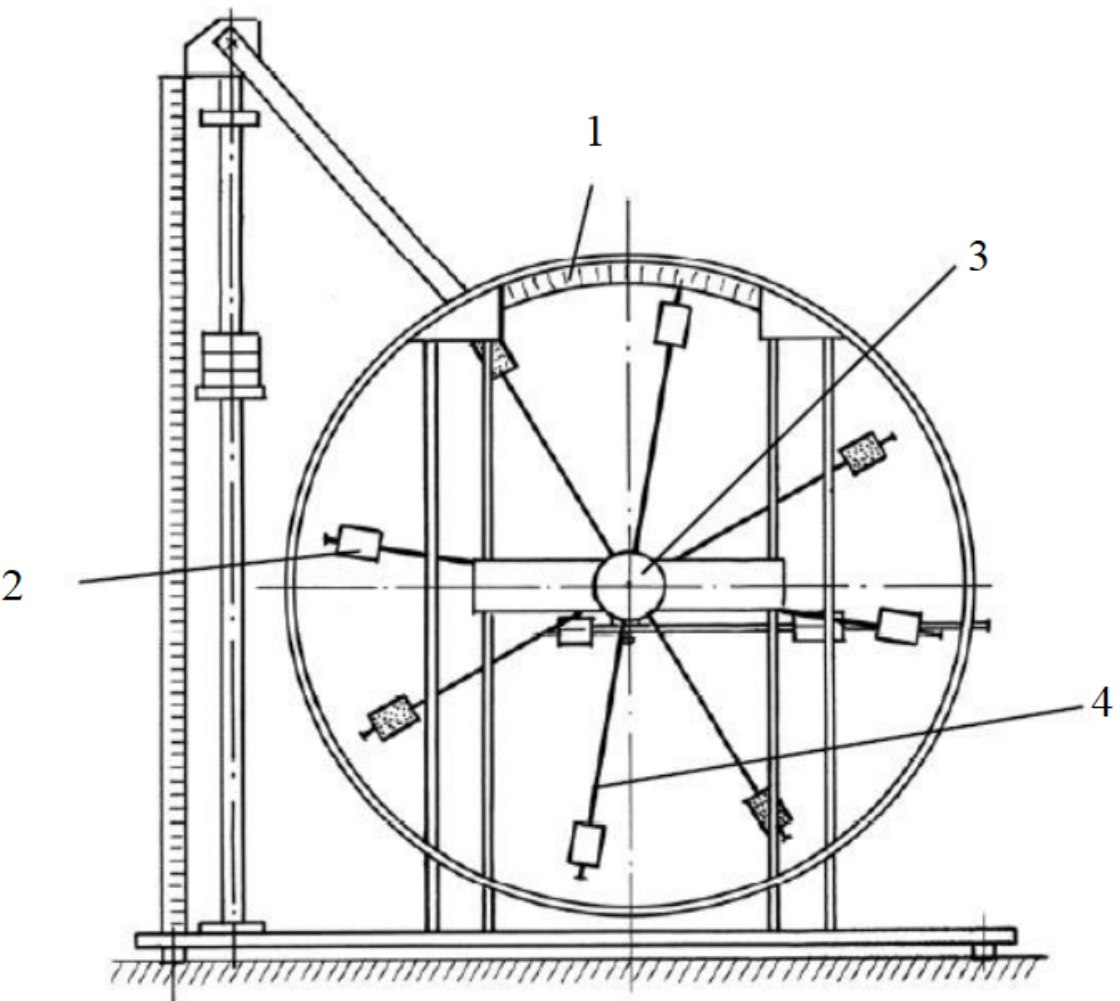
\includegraphics[width=0.5\textwidth]{img/scheme.png}
    \caption{Схема установки}
\end{figure}
